\section{Entropy Regularized Policy Gradient Methods}
\label{sec:entropy}
\subsection{Preliminaries}
Recall that the entropy regularized state value is given by 
\begin{align*}
V^\pi_\tau(s) & = \mathbb{E}_\tau\left[\sum_{t=0}^\infty \gamma^t\left({r(s_t,a_t)-\tau \log \pi(a_t|s_t)}\right)|s_0=s,\pi\right]\\
&= \mathbb{E}_\tau\left[\sum_{t=0}^\infty \gamma^t\left(r(s_t,a_t)+\tau \mathcal{H}(\pi(\cdot|s_t)\right)|s_0=s,\pi\right],
\end{align*}
where $r(s,a)\in[0,1]$ and $\mathcal{H}(p)=-\sum_ap_a\log p_a$ defines the entropy of a distribution. Moreover, the action value and the advantage function  are  defined as 
\begin{align*}
Q_\tau^\pi(s,a)=\mathbb{E}_{s'\sim P(\cdot|s,a)}\left[r(s,a)+\gamma V^\pi_\tau(s')\right]\quad\mbox{and}\quad A_\tau^\pi(s,a) = Q^\pi_\tau(s,a)-\tau\log\pi(a|s)-V_\tau^\pi(s).
\end{align*}
It can be easily seen that 
\begin{align*}\mathbb{E}_{a\sim\pi(\cdot|s)}[A^\pi_\tau(s,a)]=0.
\end{align*}


Given a policy $\pi$, the Bellman operator with entropy is defined as 
\begin{align*}
\mathcal{T}^\pi_\tau V(s) 
&=\mathbb{E}_{a\sim\pi(\cdot|s)}\mathbb{E}_{s'\sim P(\cdot|s,a)}\left[r(s,a)+\gamma V(s')-\tau\log\pi(a|s)\right]\\
&=\mathbb{E}_{a\sim \pi(\cdot|s)}\left[Q^V(s,a)\right]+\tau \mathcal{H}(\pi(\cdot|s)),
\end{align*}
where $Q^V(s,a)=\mathbb{E}_{s'\sim P(\cdot|s,a)}[r(s,a)+\gamma V(s')]$. It can be verified  that $\mathcal{T}_\tau^\pi V^\pi_\tau = V_\tau^\pi$, which is the Bellman equation for the entropy regularization case. Moreover, given two policies $\pi_1$ and $\pi_2$, one has 
\begin{align*}
\mathcal{T}_\tau^{\pi_1}V_\tau^{\pi_2}(s)-V_\tau^{\pi_2}(s) & = \mathbb{E}_{a\sim\pi_1(|s)}[Q^{\pi_2}_\tau(s,a)-\tau \log\pi_1(a|s)-V_\tau^{\pi_2}(s)]\\
&=\mathbb{E}_{a\sim\pi_1(|s)}[Q^{\pi_2}_\tau(s,a)-\tau \log\pi_2(a|s)-V_\tau^{\pi_2}(s)]\\
&\quad -\tau\mathbb{E}_{a\sim \pi_1(\cdot|s)}[\log\pi_1(a|s)-\log\pi_2(a|s)]\\
& = \mathbb{E}_{a\sim\pi_1(\cdot|s)}[A^{\pi_2}_\tau(s,a)]-\tau \mathrm{KL}(\pi_1(\cdot|s)\|\pi_2(\cdot|s)).
\end{align*}
Similar to the non-entropy case, the performance difference of two policies can also be given in terms of $\mathcal{T}_\tau^{\pi_1}V_\tau^{\pi_2}(s)-V_\tau^{\pi_2}(s)$, which can be verified directly.
\begin{lemma}[Performance difference lemma]\label{lem:entropyPDL} Given two policies $\pi_1$ and $\pi_2$, there holds 
\begin{align*}
V^{\pi_1}_\tau(\rho)-V^{\pi_2}_\tau(\rho)=\frac{1}{1-\gamma}\mathbb{E}_{s\sim d_\rho^{\pi_1}}\left[\mathcal{T}_\tau^{\pi_1}V_\tau^{\pi_2}(s)-V_\tau^{\pi_2}(s)\right].
\end{align*}
\end{lemma}


In contrast to the case without entropy, the Bellman optimality operator with entropy is defined as 
\begin{align*}
\mathcal{T}_\tau V(s)=\max_\pi\mathbb{E}_{a\sim\pi(\cdot|s)}\mathbb{E}_{s'\sim P(\cdot|s,a)}[r(s,a)-\tau\log\pi(a|s)+\gamma V(s')]=\tau\log\|\exp(Q^V(s,\cdot)/\tau)\|_1,
\end{align*}
where $Q^V(s,a)$ is defined as above. Moreover, the optimal soft PI policy (or softmax policy), at which the maximum is achieved, is given by 
\begin{align*}
\pi^{\mathrm{spi}}(\cdot|s) = \frac{\exp(Q^V(s,\cdot)/\tau)}{\|\exp(Q^V(s,\cdot)/\tau)\|_1}.
\end{align*}
Note that the Bellman operator and the optimal Bellman operator also satisfy the $\gamma$-contraction property in the entropy case:
\begin{align*}
\left\| \calT^\pi_\tau V_1 - \calT^\pi_\tau V_2 \right\|_\infty \leq \gamma \cdot \left\| V_1 - V_2 \right\|_\infty\quad \mbox{and}\quad\left\| \calT_\tau V_1 - \calT_\tau V_2 \right\|_\infty \leq \gamma \cdot \left\| V_1 - V_2 \right\|_\infty.
\end{align*}

In this section, we will let $V_\tau^*$ and $Q_\tau^*$ be the optimal entropy regularized state and action values, with the optimal policy denoted by $\pi^{*}$ (unique). One can immediately see that the first inequality in Lemma~\ref{lem:QV-relation} still holds: 
\begin{align*}
\|Q_\tau^\pi-Q^*_\tau\|_\infty\leq \gamma\cdot \|V_\tau^*-V_\tau^\pi\|_\infty.
\end{align*}
Moreover, $V_\tau^*$ satisfies the Bellman optimality equation $\mathcal{T}_\tau V_\tau^*=V_\tau^*$. It can also be shown that \cite{Nachum2017softPI}
\begin{align*}
\forall s\in\calS, \; a\in\calA: \quad V^*_\tau(s) = Q^*_\tau(s,a) - \tau \log (\pi^*(a|s)),
\end{align*}
which is equivalent to 
\begin{align*}
    \forall s\in\calS, \; a\in\calA: \quad A^*_\tau(s,a) =Q^*_\tau(s,a) - V^*_\tau(s) - \tau \log (\pi^{*}(a|s))= 0.\numberthis\label{eq:opteq}
\end{align*}
In addition, given a policy $\pi$, one has
\begin{align*}
\mathcal{T}_\tau V^{\pi}_\tau(s)-V^\pi_\tau(s) &= \tau\log\|\exp(Q^\pi_\tau(s,\cdot)/\tau)\|_1 - V^\pi_\tau(s)\\
& = Q^\pi_\tau(s,a)-\tau \log \pi^{\mathrm{spi}}(a|s) -V^\pi_\tau(s),\quad\forall a,\\
& = \sum_a \pi(a|s)\left(Q^\pi_\tau(s,a)-\tau \log \pi^{\mathrm{spi}}(a|s) -V^\pi_\tau(s)\right)\\
& = \tau\sum_a \pi(a|s)(\log \pi(a|s)-\log \pi^{\mathrm{spi}}(a|s))\\
& = \tau \mathrm{KL}\left(\pi(\cdot|s)\|\pi^{\mathrm{spi}}(\cdot|s)\right),%\numberthis\label{eq:refneeded1}
\end{align*}
where $\pi^{\mathrm{spi}}(\cdot|s)$ is obtained through $Q_\tau^\pi(s,a)$, and  the fourth equality follows from $\mathbb{E}_{a\sim\pi(\cdot|s)}[Q^\pi_\tau(s,a)-\tau\log\pi(a|s)-V^\pi_\tau(s)]=0$.

Apart from Lemma~\ref{lem:entropyPDL}, there are several other lemmas that will be used throughout this section. The first one can be verified directly. 
\begin{lemma}\label{lem:entropy-value-bound}
For any policy $\pi$, one has 
\begin{align*}
V_\tau^\pi(s)\in\left[0,\frac{1+\tau\log|\mathcal{A}|}{1-\gamma}\right]\quad\mbox{and}\quad Q_\tau^\pi(s,a)\in\left[0,\frac{1+\gamma\,\tau\log|\mathcal{A}|}{1-\gamma}\right].
\end{align*}
\end{lemma}

The following lemma can be viewed as the entropy analogue of Lemma~\ref{lem:bsk-bounds}, which characterizes the optimality of an policy in the value space based on the KL-divergence in the policy space. This lemma can be proved easily by applying Lemma~\ref{lem:entropyPDL} to $-\left(V_\tau^\pi(\rho)-V_\tau^*(\rho)\right)$ and then using the fact $A_\tau^*(s,a)=0$ in \eqref{eq:opteq}.
\begin{lemma}[\protect{\cite[Lemma~26]{Mei_Xiao_Szepesvari_Schuurmans_2020}}]\label{lem:KL-opt}
For any policy $\pi$ and $\rho\in\Delta(\mathcal{S})$, there holds
\begin{align*}
V_\tau^*(\rho) - V_\tau^\pi(\rho)=\frac{\tau}{1-\gamma}\mathbb{E}_{s\sim d_\rho^\pi}\left[\mathrm{KL}(\pi(\cdot|s)\|\pi^*(\cdot|s))\right].
\end{align*}
\end{lemma}

Letting  $\{\pi^k\}$ be a sequence of policies, we will use the shorthand notation 
$V_\tau^k$ and $\mathcal{T}_\tau^{k+1}$ for $V_\tau^{\pi^k}$ and $\mathcal\mathcal{T}_\tau^{\pi^{k+1}}$, respectively.  The next lemma is an entropy regularization version of Theorem~\ref{thm:linear-infinity}, and the proof details  are thus omitted.
\begin{lemma}\label{lem:entroy-convergence-lemma}
If $\mathcal{T}_\tau^{k+1}V_\tau^k(s)-V_\tau^k(s)\geq C_k\left(\mathcal{T}_\tau V_\tau^k(s)-V_\tau^k(s)\right)$ for some $C\in(0,1)$, then 
\begin{align*}
\|V_\tau^*-V_\tau^{k+1}\|_\infty\leq  \left(1-(1-\gamma)\,C_k\right)\|V^*_\tau-V^{k}_\tau\|_\infty.
\end{align*}
\end{lemma}

%\kw{Briefly say something about $\mathcal{L}^{k+1}_k$ and $\mathcal{L}^{\max}_k$ later}, 
%other useful notation
 
 In this section, we will define $\mathcal{L}_k^{k+1}$ as 
\begin{align*}
\mathcal{L}_k^{k+1} = \frac{1}{1-\gamma}\sum_sd_\rho^*(s)\left(\mathcal{T}_\tau^{k+1}V_\tau^{k}(s)-V_\tau^{k}(s)\right),\numberthis\label{eq:entropy-Lk}
\end{align*}
and define $\mathcal{L}_k^*$ as 
\begin{align*}
\mathcal{L}_k^*=\frac{1}{1-\gamma}\sum_sd_\rho^*(s)\left(\mathcal{T}_\tau^*V_\tau^{k}(s)-V_\tau^{k}(s)\right),\numberthis\label{eq:entropy-Lstar}
\end{align*}
where
 $d_\rho^*$ is the visitation measure with respect to the optimal policy $\pi^*$, and $\mathcal{T}^*_\tau$ is the Bellman operator associated with  $\pi^*$.
It is clear that the following result still holds:
\begin{align*}
\mathcal{L}_k^*=V_\tau^*(\rho)-V_\tau^k(\rho).
\end{align*}
As in the non-entropy case, we consider minimizing $V_\tau^{\pi_\theta}(\mu)$ for fixed $\mu$ with $\tilde{\mu}=\min_s\mu(s)>0$ and the state value error $V_\tau^*(\rho)-V_\tau^k(\rho)$ will be evaluated for  an arbitrary $\rho$ with $\tilde{\rho}=\min_s\rho(s)>0$.
%%%%%%%%%%%%%%%%%%%%%%
%%%%%%%%%%%%%%%%%%%%%%
\subsection{Entropy Softmax PG}
%{\color{red} (add parameterization update, used in proof of global convergence)} For the entropy regularization case,  the update of policy gradient  under the softmax parameterization is overall similar to that for the case without entropy, but with $A^k(s,a)$ in REF being replace by $A_\tau^k(s,a)$:
Under softmax parameterization, the policy gradient of $V^{\pi_\theta}(\mu)$ with respect to $\theta$ is overall similar to that of the non-entropy case in \eqref{eq:softmax-gradient}, but with $A^{\pi_\theta}(s,a)$ being replace by $A_\tau^{\pi_\theta}(s,a)$:
  \begin{align*}
        \frac{\partial V_\tau^{\pi_\theta}(\mu)}{\partial \theta_{s,a}} = \frac{1}{1-\gamma} d^{\pi_\theta}_\mu(s)\, \pi_\theta(a|s) A_\tau^{\pi_\theta}(s,a).\numberthis\label{eq:entropy-softmax-pg-expression}
    \end{align*}
    Then the update of entropy softmax PG with constant step size in the parameter space is given by 
\begin{align*}
\theta_{s,a}^{k+1} = \theta^k_{s,a}+\eta_s\,\pi^k_{s,a}A^k_\tau(s,a),
\end{align*}
while in the policy space is given by
\begin{align*}
\pi^{k+1}_{s,a}\propto \pi^k_{s,a}\exp\left(\eta_s\,\pi^k_{s,a}A^k_\tau(s,a)\right),
\end{align*}
where $\eta_s=\frac{\eta}{1-\gamma}d_\mu^k(s)$ and $d_\mu^k$ is the visitation measure under the policy $\pi^k$. Again, we will use the shorthand notation $\pi^k_{s,a}$ for $\pi^k(a|s)$ and use $\pi^k_s$ for $\pi^k(\cdot|s)$ whenever it is convenient.  As in the case for softmax PG, we  let
\begin{align*}
\hat{A}^k_\tau(s,a)=\pi^k(a|s)A^k_\tau(s,a).
\end{align*}
It is evident that $\sum_a\hat{A}^k_\tau(s,a)=0$. Moreover, we have the following result, whose proof can be found in  Appendix~\ref{sec:proof-bound-Atau}.
\begin{lemma}\label{lem:bound-Atau}
For any policy $\pi$, one has 
\begin{align*}
\|\hat{A}_\tau^\pi\|_\infty\leq \frac{1+\tau\log|\mathcal{A}|}{1-\gamma}.
\end{align*}
\end{lemma}


In this subsection, we  establish the linear convergence of entropy softmax PG for a wider range of constant step sizes than that can be allowed in \cite{Mei_Xiao_Szepesvari_Schuurmans_2020} based on the similar analysis technique used for softmax PG in Section~\ref{sec:softmaxPG}. The following inequalities regarding the distances of two softmax policies will be used.
\begin{lemma}[\protect{\cite[Lemma~27]{Mei_Xiao_Szepesvari_Schuurmans_2020}} \textup{and} \protect{\cite[Section~A.2]{Cen_Cheng_Chen_Wei_Chi_2022}}]\label{lem:KL-softmax}
Let $\pi_\theta=\mathrm{softmax}(\theta)$ and $\pi_{\theta'}=\mathrm{softmax}(\theta')$ be two softmax policies. Then 
\begin{align*}
\mathrm{KL}(\pi_\theta\|\pi_{\theta'})\leq \frac{1}{2}\|\theta-\theta'-c\cdot \bm{1}\|_\infty^2
\end{align*}
for any constant $c\in\R$. In particular, taking $c=\log \|\exp(\theta)\|_1-\log \|\exp(\theta')\|_1$ yields 
\begin{align*}
\mathrm{KL}(\pi_\theta\|\pi_{\theta'})\leq \frac{1}{2}\|\log\pi_\theta-\log\pi_{\theta'}\|_\infty^2.
\end{align*}
Moreover, one has
\begin{align*}
\|\log\pi_\theta-\log\pi_{\theta'}\|_\infty\leq 2\|\theta-\theta'\|_\infty.
\end{align*}
\end{lemma}
As in the non-entropy case, the analysis begins with a state-wise improvement lower bound in terms of $\max_a|\hat{A}_\tau^k(s,a)|$.
%%%%%%%%%%%%%%%
\begin{lemma}[Improvement Lower Bound]\label{lem:entropy-lower-bound}
    For entropy softmax PG with step size $\eta>0$,
\begin{align*}
\mathcal{T}_\tau^{k+1}V_\tau^k(s)-V_\tau^k(s)\geq \eta\,\tilde{\mu}\left[\exp\left(-\frac{2\,\eta\,(1+\tau\log|\mathcal{A}|)}{(1-\gamma)^2}\right)-\frac{\tau\,\eta}{2(1-\gamma)}\right]\,\max_a|\hat{A}_\tau^k(s,a)|^2.
\end{align*}
Moreover, there exists a unique solution to 
\begin{align*}
    \exp\left(-\frac{2\,x\,(1+\tau\log|\mathcal{A}|)}{(1-\gamma)^2}\right)-\frac{\tau\,x}{2(1-\gamma)}=0,
\end{align*}
denoted $\beta$, such that $\mathcal{T}_\tau^{k+1}V_\tau^k(s)-V_\tau^k(s)\geq 0$ for $\eta\in(0,\beta)$.
\end{lemma}
\begin{proof}
    Recall that
\begin{align*}
\mathcal{T}_\tau^{k+1}V_\tau^k(s)-V_\tau^k(s)=\sum_a\pi^{k+1}(a|s)A^k_\tau(s,a)-\tau\,\mathrm{KL}(\pi^{k+1}(\cdot|s)\|\pi^k(\cdot|s)).
\end{align*}
For the KL part, setting $c=0$ in Lemma~\ref{lem:KL-softmax} gives
\begin{align*}
\mathrm{KL}(\pi^{k+1}(\cdot|s)\|\pi^k(\cdot|s))&\leq \frac{1}{2}\|\theta^{k+1}_s-\theta^k_s\|_\infty^2=\frac{1}{2}\|\eta_s\,\hat{A}^k_\tau(s,\cdot)\|_\infty^2\\
&=\frac{1}{2}(\eta_s)^2\max_a|\hat{A}_\tau^k(s,a)|^2.
\end{align*}
For the first term, letting $Z_s^k = \mathbb{E}_{a\sim \pi^k(\cdot|s)}\left[\exp\left(\eta_s\,\hat{A}^k_\tau(s,a)\right)\right]$ and $\alpha=(1+\tau\log|\mathcal{A}|)/(1-\gamma)$, one has 
\begin{align*}
&\sum_a\pi^{k+1}(a|s)A^k_\tau(s,a)\\
&=\frac{1}{Z_s^k}\sum_a \hat{A}_\tau^k(s,a)\exp\left(\eta_s\,\hat{A}_\tau^k(s,a)\right)\\
&=\frac{|\mathcal{A}|}{Z_s^k}\mathrm{Cov}_{a\sim U}\left(\hat{A}_\tau^k(s,a),\exp\left(\eta_s\,\hat{A}_\tau^k(s,a)\right)\right)\\
&=\frac{1}{2\,Z_s^k|\mathcal{A}|}\sum_{a,a'}\left[\hat{A}_\tau^k(s,a)-\hat{A}_\tau^k(s,a')\right]\left[\exp\left(\eta_s\,\hat{A}_\tau^k(s,a)\right)-\exp\left(\eta_s\,\hat{A}_\tau^k(s,a')\right)\right]\\
&=\frac{1}{Z_s^k|\mathcal{A}|}\sum_{\hat{A}_\tau^k(s,a)>\hat{A}_\tau^k(s,a')}\left[\hat{A}_\tau^k(s,a)-\hat{A}_\tau^k(s,a')\right]\left[\exp\left(\eta_s\,\hat{A}_\tau^k(s,a)\right)-\exp\left(\eta_s\,\hat{A}_\tau^k(s,a')\right)\right]\\
&=\frac{1}{Z_s^k|\mathcal{A}|}\sum_{\hat{A}_\tau^k(s,a)>\hat{A}_\tau^k(s,a')}\exp\left(\eta_s\,\hat{A}_\tau^k(s,a')\right)\left[\hat{A}_\tau^k(s,a)-\hat{A}_\tau^k(s,a')\right]\left[\exp\left(\eta_s\left(\hat{A}_\tau^k(s,a)-\hat{A}_\tau^k(s,a')\right)\right)-1\right]\\
&\geq\frac{\exp(-\eta_s\,\alpha)}{Z_s^k|\mathcal{A}|}\sum_{\hat{A}_\tau^k(s,a)>\hat{A}_\tau^k(s,a')}\left[\hat{A}_\tau^k(s,a)-\hat{A}_\tau^k(s,a')\right]\left[\exp\left(\eta_s\left(\hat{A}_\tau^k(s,a)-\hat{A}_\tau^k(s,a')\right)\right)-1\right]\\
&\geq \frac{\eta_s\exp(-\eta_s\,\alpha)}{Z_s^k|\mathcal{A}|}\sum_{\hat{A}_\tau^k(s,a)>\hat{A}_\tau^k(s,a')}\left[\hat{A}_\tau^k(s,a)-\hat{A}_\tau^k(s,a')\right]^2\\
&\geq \frac{\eta_s\exp(-2\eta_s\,\alpha)}{|\mathcal{A}|}\sum_{\hat{A}_\tau^k(s,a)>\hat{A}_\tau^k(s,a')}\left[\hat{A}_\tau^k(s,a)-\hat{A}_\tau^k(s,a')\right]^2\\
&\geq \frac{\eta_s\exp(-2\eta_s\,\alpha)}{2\,|\mathcal{A}|}\sum_{a,a'}\left[\hat{A}_\tau^k(s,a)-\hat{A}_\tau^k(s,a')\right]^2\\
&=\eta_s|\mathcal{A}|\exp(-2\eta_s\,\alpha)\mathrm{Var}_{a\sim u}\left(\hat{A}_\tau^k(s,a)\right)\\
&=\eta_s\exp(-2\eta_s\,\alpha)\sum_a \hat{A}_\tau^k(s,a)^2\\
&\geq \eta_s\exp(-2\eta_s\,\alpha)\max_a \hat{A}_\tau^k(s,a)^2,
\end{align*}
where the third inequality follows from $Z_s^k\leq \exp(\eta_s\max_a\hat{A}_\tau^k(s,a))\leq \exp(\eta_s\,\alpha)$.

Combining the above two bounds together yields
\begin{align*}
\mathcal{T}_\tau^{k+1}V_\tau^k(s)-V_\tau^k(s)&\geq \eta_s\left(\exp(-2\eta_s\,\alpha)-\frac{\tau}{2}\eta_s\right)\max_a |\hat{A}_\tau^k(s,a)|^2\\
&\geq\eta\,\tilde{\mu}\left[\exp\left(-\frac{2\eta\,\alpha}{1-\gamma}\right)-\frac{\tau\,\eta}{2(1-\gamma)}\right]\max_a |\hat{A}_\tau^k(s,a)|^2.
\end{align*}
where the second line follows from $\eta\,\tilde{\mu}\leq\eta_s\leq\eta/(1-\gamma)$. The proof of the first claim is now complete, and the second claim can be verified directly.
\end{proof}

Based on the improvement lower bound we can first establish the global convergence of entropy softmax PG for $\eta\in(0,\beta)$.  The key is to show that the limit of $\pi^k_{s,a}$ for any $(s,a)$ exists. Once it is done, the proof follows closely the one for Lemma~16 in \cite{Mei_Xiao_Szepesvari_Schuurmans_2020}. The proof of this result is deferred  to Appendix~\ref{sec:proof-entropyPG-global}.
\begin{lemma}[Global Convergence]\label{lem:entropyPG-global}
   For any $\eta\in(0,\beta)$, the value sequence $\{ V^k_\tau(\rho) \}$ produced by entropy softmax PG converges to the optimal value, 
    \begin{align*}
        \forall \, s\in\calS: \quad \lim_{k\to\infty} V^k_\tau(s) = V^*_\tau(s).
    \end{align*}
\end{lemma}

Note that the following result can be obtained as a byproduct of  the proof of Lemma~\ref{lem:entropyPG-global}:
\begin{align*}
    \kappa:=\inf_{k\geq 0}\min_{s,a}\pi^k_{s,a}>0.
\end{align*}
Now we are in the position to show the linear convergence of entropy softmax PG.
\begin{theorem}[Linear Convergence]\label{thm:entropyPG-linear}
    For any constant step size $\eta\in(0,\beta)$, entropy softmax PG converges linearly,
    \begin{align*}
        \|V_\tau^*-V_\tau^k\|_\infty\leq
        \left(1-(1-\gamma)\eta\,\tilde{\mu}\,\tau\,\kappa^2\left[2\exp\left(-\frac{2\,\eta\,(1+\tau\log|\mathcal{A}|)}{(1-\gamma)^2}\right)-\frac{\tau\,\eta}{(1-\gamma)}\right]\right)^k\|V_\tau^*-V_\tau^k\|_\infty.
    \end{align*}
\end{theorem}
\begin{proof}
Define 
    \begin{align*}
\pi^{k,\mathrm{spi}}(\cdot|s) = \frac{\exp\left(Q^k_\tau(s,\cdot)/\tau\right)}{\|\exp\left(Q^k_\tau(s,\cdot)/\tau\right\|_1}.
\end{align*}
By Lemma~\ref{lem:KL-softmax}, one has
\begin{align*}
\mathcal{T}_\tau V^k(s)-V^k(s) & =\tau\,\mathrm{KL}(\pi^k(\cdot|s)\|\pi^{k,\mathrm{spi}}(\cdot|s))\\
&\leq \frac{\tau}{2}\left\|\theta_s^k-Q^k_\tau(s,\cdot)/\tau+c\cdot \bm{1}\right\|_\infty^2\\
&=\frac{\tau}{2}\|\log\pi^k(\cdot|s)-Q_\tau^k(s,\cdot)/\tau+(c-\log\|\exp(\theta_s^k)\|_1)\cdot \bm{1}\|_\infty^2.
\end{align*}
Setting $c=\log\|\exp(\theta_s^k)\|_1+V_\tau^k(s)/\tau$  yields that 
\begin{align*}
\mathcal{T}_\tau V^k(s)-V^k(s)& \leq \frac{1}{2\,\tau}\|A^k_\tau(s,\cdot)\|_\infty^2\\
&\leq \frac{1}{2\,\tau\,\kappa^2}\max_a|\hat{A}^k_\tau(s,a)|^2, 
\end{align*}
Combining it with the improvement lower bound and then applying Lemma~\ref{lem:entroy-convergence-lemma}
completes the proof.
\end{proof}

\begin{remark}
    In \textup{\cite{Mei_Xiao_Szepesvari_Schuurmans_2020}}, the linear convergence of entropy softmax PG has been established for $\eta\in(0,2\alpha]$ with $\alpha=(1-\gamma)^3 / (8+\tau(4+8\log |\calA|))$, with the rate at $\alpha$ being given by
    \begin{align*}
        V^*_\tau(\rho) - V^k_\tau(\rho) 
        \leq \frac{1}{\tilde{\mu}} \cdot \frac{1+\tau \log |\calA|}{(1-\gamma)^2} \cdot \exp \left( -(k-1) \cdot \frac{(1-\gamma)\, \tau\, \alpha}{|\calS|} \cdot \tilde{\mu}\, \kappa^2 \left\| \frac{d^*_\mu}{\mu} \right\|_\infty^{-1} \right).
        \numberthis\label{eq:mei-entropy}
    \end{align*}
    Indeed one can show that $2\alpha<\beta$. Thus, our result is applicable for a wider range of constant step sizes. To see this, first note that 
    \begin{align*}
        \alpha = \frac{(1-\gamma)^3}{8+\tau(4+8\log |\calA|)} < \frac{(1-\gamma)^3}{8+ 8\tau \log |\calA|} = \frac{(1-\gamma)^2}{8\,c} := \alpha^\prime,
    \end{align*}
    where $c = (1+\tau \log |\calA|) / (1-\gamma)$. We have
    \begin{align*}
        \exp\left( -\frac{4\alpha^\prime}{1-\gamma} c \right) - \frac{\tau\alpha^\prime}{(1-\gamma)} &= \exp \left( -\frac{1-\gamma}{2} \right) - \frac{\tau(1-\gamma)}{8\,c} \\
        &\geq 1- \frac{1-\gamma}{2} - \frac{\tau(1-\gamma)}{8\,c} \\
        &= 1- \frac{(1-\gamma)(4 + \tau/c)}{8} \\
        &>0,
    \end{align*}
    where the last inequality utilizes  $\tau / c < 2(1-\gamma)$ for $|\calA| >1$. By the monotonically decreasing property of the function $\exp\left( -\frac{2\,x}{1-\gamma} c \right) - \frac{\tau\,x}{2(1-\gamma)}$, it can be concluded that $2\alpha < 2\alpha^\prime < \beta$, i.e. we provide a wider range of step sizes for entropy softmax PG to converge linearly. 
    
    Furthermore, one can verify that 

    \begin{align*}
        \exp\left( -\frac{2\alpha}{1-\gamma} c \right) - \frac{\tau\alpha}{2(1-\gamma)} \geq \exp\left( -\frac{2\alpha^\prime}{1-\gamma} c \right) - \frac{\tau\alpha^\prime}{2(1-\gamma)} \geq 1 - \frac{(1-\gamma)(4+\tau/c)}{16} > \frac{1}{2}. \numberthis \label{eq:remark-ent-softmax-pg}
    \end{align*}
    Therefore plugging $\alpha = (1-\gamma)^3 / (8+\tau(4+8\log |\calA|))$ into Theorem~\ref{thm:entropyPG-linear} gives
    \begin{align*}
        V^*_\tau(\rho) - V^k_\tau(\rho) \leq \left\| V^*_\tau - V^k_\tau \right\|_\infty &\leq \left( 1-(1-\gamma)\, \alpha\, \tilde{\mu}\, \kappa^2 \left[ 2\exp\left( -\frac{2\,\alpha}{1-\gamma} c \right) - \frac{\tau\alpha}{1-\gamma} \right]\right)^k \cdot \left\| V^*_\tau - V^0_\tau \right\|_\infty \\
        &\leq \frac{1+\tau\log |\calA|}{1-\gamma} \cdot \left[ 1-(1-\gamma)\,  \alpha \,\tilde{\mu}\, \tau\, \kappa^2 \right]^k \\
        &\leq \frac{1+\tau\log |\calA|}{1-\gamma} \cdot \exp \left( -k \cdot (1-\gamma)\, \alpha\, \tilde{\mu}\, \tau\, \kappa^2 \right),
    \end{align*}
    where the second inequality is due to Lemma~\ref{lem:entropy-value-bound} and equation~\eqref{eq:remark-ent-softmax-pg}. 
    Compared with \eqref{eq:mei-entropy}, our result is clearly better. 
\end{remark}

\begin{remark}
    For softmax PG, we have established its convergence   for any constant step size \textup{(}though with sublinear convergence rate\textup{)}. For entropy softmax PG, the convergence can only be guaranteed for the step size over a finite interval. Thus, one may wonder whether the convergence of entropy softmax PG can be established for any constant step size. To investigate this issue, numerical test has been conducted on a random MDP,  and the result suggests entropy softmax PG does not converge for a large step size, see Figure~\ref{fig:entropypg}. In the test,   the rewards for the state-action pairs and the entries of the transition probability matrix are generated through a uniform distribution over $\left(0,1\right)$. We then re-scale each row of the transition probability matrix to obtain a stochastic matrix. 
\end{remark}

\begin{figure}[ht!]
    \centering
    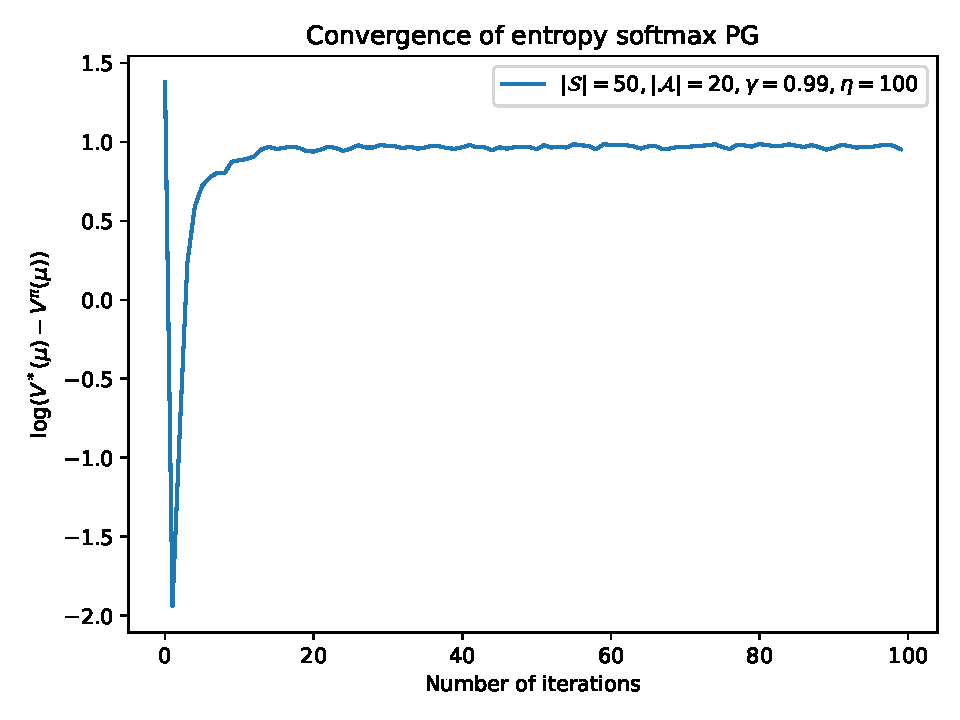
\includegraphics[width=0.5\textwidth]{EntropyPG.pdf}
    \caption{A random MDP example which shows entropy softmax PG does not converge for large step size. }
    \label{fig:entropypg}
\end{figure}
%%%%%%%%%%%%%%%%%%%%%%
%%%%%%%%%%%%%%%%%%%%%%
\subsection{Entropy  Softmax NPG}
As for softmax NPG, we present the update of  the entropy  softmax NPG  directly in the policy space,  given by
\begin{align*}
\pi^{k+1}_{s,a}&\propto \pi^k_{s,a}\exp\left(\frac{{\eta}}{{\eta}\tau+1}A^k_\tau(s,a)\right)\\
&\propto \exp\left(\frac{\eta}{\eta\tau+1}Q^k_\tau(s,a)+\frac{1}{\eta\tau+1}\log \pi^k_{s,a}\right),
\numberthis\label{eq:entropyNPG}
\end{align*}
where $\eta>0$ is the step size.
Entropy softmax NPG coincides with the following entropy regularized policy mirror ascent update:
\begin{align*}
\pi_s^{k+1} = \argmax_{p\in\Delta(\mathcal{A})}\left\{{\eta}\left(\langle Q^{k}_\tau(s,\cdot),p\rangle + \tau \mathcal{H}(p)\right)-\mathrm{KL}(p\|\pi^k_s)\right\}.
\end{align*}
In addition, when $\eta\rightarrow\infty$, \eqref{eq:entropyNPG} reduces to soft PI
\begin{align*}
    \pi^{k+1}_{s,a}&\propto \pi^k_{s,a}\exp\left(A_\tau^k(s,a)/\tau\right)\\
    &\propto \exp\left(Q_\tau^k(s,a)/\tau\right)\numberthis\label{eq:softPI}
\end{align*}
 The linear convergence of entropy  softmax NPG in terms of infinity norm has been established in  \cite[Theorem~1]{Cen_Cheng_Chen_Wei_Chi_2022}. 
 
\begin{theorem}[\protect{\cite[Theorem 1]{Cen_Cheng_Chen_Wei_Chi_2022}}] \label{theorem: ent_npg: linear convergence of log probability}
For any constant size $\eta>0$, the sequence generated by  entropy  softmax NPG satisfies\footnote{Note that there is a change of variable between the step size used in \eqref{eq:entropyNPG} and that used in \cite{Cen_Cheng_Chen_Wei_Chi_2022}.}
\begin{align*}
\|Q_\tau^*-Q_\tau^k\|_\infty&\leq C_1\gamma\left( 1-\left( 1-\gamma \right) \frac{\eta \tau}{\eta \tau +1} \right) ^{k-1},\numberthis\label{eq:chen-npg-Q}\\
\left\| \log \pi ^*-\log \pi ^k \right\| _{\infty}&\le \frac{2C_1}{\tau}\left( 1-\left( 1-\gamma \right) \frac{\eta \tau}{\eta \tau +1} \right) ^{k-1}\numberthis\label{eq:chen-npg-pi},
\end{align*}  
where $\pi^*$ is the optimal policy for the entropy regularized RL problem, $Q^*_\tau$ is the corresponding optimal action value function, and $
C_1:=\left\| Q_{\tau}^{*}-Q_{\tau}^{0} \right\| _{\infty}+2\tau \left( 1-\frac{\eta \tau}{1+\eta \tau} \right) \left\| \log \pi ^*_\tau-\log \pi ^0 \right\| _{\infty}$.
\end{theorem}
\noindent It is also noted after \cite[Theorem 1]{Cen_Cheng_Chen_Wei_Chi_2022} that, since 
\begin{align*}
V_\tau^*(s)-V_\tau^k(s) &= \mathbb{E}_{a\sim \pi^k(\cdot|s)}\left[(Q^*_\tau(s,a)-\tau\log\pi^*(a|s))-(Q^k_\tau(s,a)-\tau\log\pi^k(a|s))\right]\\
&\leq \tau \|\log \pi^*-\log \pi^k\|_\infty+\|Q_\tau^*-Q_\tau^k\|_\infty,
\end{align*}
the linear convergence in terms of the entropy regularized state value follows immediately:
\begin{align*}
\|V_\tau^*-V_\tau^k\|_\infty\leq(2+\gamma) C_1 \left( 1-\left( 1-\gamma \right) \frac{\eta \tau}{\eta \tau +1} \right) ^{k-1}.
\end{align*}
We first show that a simple application of  Lemma~\ref{lem:KL-opt} can improve the  convergence rate for the state value from $ 1-\left( 1-\gamma \right) \frac{\eta \tau}{\eta \tau +1}  $ to $\left( 1-\left( 1-\gamma \right) \frac{\eta \tau}{\eta \tau +1} \right)^2$.
\begin{theorem}\label{thm:entropyNPG-improvement}
For any constant step size $\eta>0$, the value sequence $\{ V^k_\tau(\rho) \}$ produced by entropy softmax NPG satisfies 
\begin{align*}
\left\|V_\tau^*-V^k_\tau\right\|_\infty \leq \frac{2\,C_1^2}{(1-\gamma)\,\tau}\left( 1-\left( 1-\gamma \right) \frac{\eta\, \tau}{\eta\, \tau +1} \right) ^{2\,(k-1)},\numberthis\label{eq:entropy-npg-global-rate}
\end{align*}
where $C_1$ is defined as above.
\end{theorem}
\begin{proof}
It follows from Lemma~\ref{lem:KL-softmax} that 
\begin{align*}
\mathrm{KL}(\pi^k(\cdot|s)\|\pi_\tau^*(\cdot|s))&\leq \frac{1}{2}\|\log\pi^k(\cdot|s)-\log\pi_\tau^*(\cdot|s)\|_\infty^2\leq \frac{1}{2}\|\log\pi^k-\log\pi_\tau^*\|_\infty^2\\
&\leq\frac{2C_1^2}{\tau^2}\left( 1-\left( 1-\gamma \right) \frac{\eta \tau}{\eta \tau +1} \right) ^{2(k-1)},
\end{align*}
where the last inequality follows from the inequality \eqref{eq:chen-npg-pi}. Therefore,
\begin{align*}
V_\tau^*(\rho)-V^k_\tau(\rho) & = \frac{\tau}{1-\gamma}\mathbb{E}_{s\sim d_\rho^k}\left[\mathrm{KL}\left(\pi^k(\cdot|s)\|\pi_\tau^*(\cdot|s)\right)\right]\\
&\leq \frac{2\,C_1^2}{(1-\gamma)\,\tau}\left( 1-\left( 1-\gamma \right) \frac{\eta\,\tau}{\eta \,\tau +1} \right) ^{2(k-1)}.
\end{align*}
Noting that $\rho$ can be an arbitrary distribution over $\mathcal{S}$, the proof is complete.
\end{proof}



For the special Soft PI case ($\eta\rightarrow\infty$), the local quadratic convergence rate has also been established in \cite[Theorem~3]{Cen_Cheng_Chen_Wei_Chi_2022}. Next, we are going to  provide an elementary analysis of the local quadratic convergence of soft PI with improved rate  and without additional assumption on the stationary distribution under the optimal policy $\pi^*$. To this end, we first  establish the following convergence property of soft PI.
\begin{lemma}\label{lem:softpi}
    For any $t\ge 0$, the state value errors of soft PI satisfy 
    \begin{align*}
        \forall\,k\geq t:\quad \|V_\tau^*-V_\tau^k\|_\infty\leq \frac{2\,\tau(1-\gamma)}{\gamma^2}\exp\left(2^t\log\left(a_0\cdot\gamma^{k-t}\right)\right),\numberthis\label{eq:softpi01}
    \end{align*}
    where $a_0:=\displaystyle{\frac{1}{2\tau}\frac{\gamma ^2}{\left( 1-\gamma \right)}}\left\| V_{\tau}^{*}-V_{\tau}^{0} \right\| _{\infty}$.
\end{lemma}
\begin{proof}
    Noting that in soft PI,
    $
    \pi_s^{k+1} = \mathrm{softmax}\left(Q_\tau^k(\cdot|s)/\tau\right),
    $
    the application of Lemma~\ref{lem:KL-softmax} yields that 
    \begin{align*}
        \mathrm{KL}(\pi_s^{k+1}\|\pi_s^*) \leq \frac{1}{2\,\tau^2}\|Q^k_\tau(\cdot|s)-Q^*_\tau(\cdot|s)\|_\infty^2\leq \frac{1}{2\,\tau^2}\|Q^k_\tau-Q^*_\tau\|_\infty^2\leq \frac{\gamma^2}{2\,\tau^2}\|V^k_\tau-V^*_\tau\|_\infty^2.
    \end{align*}
    Then it follows from Lemma~\ref{lem:KL-opt} that 
    \begin{align*}
        V_\tau^*(\rho)-V_\tau^{k+1}(\rho)&=\frac{\tau}{1-\gamma}\mathbb{E}_{s\sim d_\rho^{k+1}}\left[\mathrm{KL}(\pi_s^{k+1}\|\pi_s^*)\right]\\
        &\leq \frac{1}{2\,\tau}\frac{\gamma^2}{1-\gamma}\|V^k_\tau-V^*_\tau\|_\infty^2.
    \end{align*}
    Since this inequality holds for any $\rho$, one has
    \begin{align*}
       \forall\,k\geq 0:\quad  \|V_\tau^*-V_\tau^{k+1}\|_\infty\leq \frac{1}{2\,\tau}\frac{\gamma^2}{1-\gamma}\|V^k_\tau-V^*_\tau\|_\infty^2.\numberthis\label{eq:softpi02}
    \end{align*}

Next, we will proceed the proof by induction on $t$. When $t=0$, by the $\gamma$-contraction property of $\mathcal{T}_\tau$, it can be shown that \cite{Nachum2017softPI}
\begin{align*}
    \|V_\tau^*-V_\tau^k\|_\infty\leq \gamma^k\|V_\tau^*-V_\tau^0\|_\infty,
\end{align*}
which coincides with \eqref{eq:softpi01}. Now suppose \eqref{eq:softpi01} holds for $t=m-1$. For $t=m$, by  \eqref{eq:softpi02}, one has 
\begin{align*}
    \forall\,k\geq m:\quad \|V_\tau^*-V_\tau^k\|_\infty&\leq  \frac{1}{2\,\tau}\frac{\gamma^2}{1-\gamma}\|V^{k-1}_\tau-V^*_\tau\|_\infty^2\\
    &\leq \frac{1}{2\,\tau}\frac{\gamma^2}{1-\gamma}\left[\frac{2\,\tau(1-\gamma)}{\gamma^2}\exp\left(2^{m-1}\log\left(a_0\cdot\gamma^{(k-1)-(m-1)}\right)\right)\right]^2\\
    &=\frac{2\,\tau(1-\gamma)}{\gamma^2}\exp\left(2^m\log\left(a_0\cdot \gamma^{k-m}\right)\right),
\end{align*}
where the second inequality follows from $k-1\geq m-1$ and the induction assumption.
\end{proof}
%%%%%%
\begin{theorem}[Local quadratic convergence of soft PI]\label{thm:softPI-quadratic}
The state value errors of soft PI satisfy 
%\begin{align*}
%\begin{cases}
%    \displaystyle{\forall\, k\geq 1:\quad \|V_\tau^*-V_\tau^k\|_\infty \leq \frac{2\,\tau(1-\gamma)}{\gamma^2}\,\gamma^{\displaystyle 2^{ k-1}}}, & \mbox{if }\displaystyle a_0\leq 1,\\
%   \\
%   \forall\, k\geq 2+\frac{\log a_0}{\log\frac{1}{\gamma}}:\quad\displaystyle\|V_\tau^*-V_\tau^k\|_\infty \leq \frac{2\,\tau(1-\gamma)}{\gamma^2}\,\gamma^{\displaystyle 2^{ k-\left(2+\frac{\log a_0}{\log\frac{1}{\gamma}}\right)}}, & \mbox{if }a_0> 1.
%\end{cases}
%\end{align*}

\begin{align*}
    \forall k\geq k_0 : \quad \|V_\tau^*-V_\tau^k\|_\infty \leq \frac{2\,\tau(1-\gamma)}{\gamma^2}\,\gamma^{\displaystyle 2^{ k-k_0}},
\end{align*}
where $k_0$ is given by
\begin{align*}
    k_0 = 
    \left\{ 
        \begin{array}{cc}
            1 & \mbox{if }a_0 \leq 1, \\
            2+\frac{\log a_0}{\log \frac{1}{\gamma}} & \mbox{if }a_0 > 1.
        \end{array}
    \right.
\end{align*}

%\begin{align*}
%    \forall\,k\geq 1:\quad  \|V_\tau^*-V_\tau^k\|_\infty \leq \frac{2\,\tau(1-\gamma)}{\gamma^2}\gamma^{2^{k-1}},\quad\mbox{if }a_0\leq 1
%\end{align*}
\end{theorem}
\begin{proof}
    In the case $a_0\leq 1$, setting $t=k-1$ in \eqref{eq:softpi01} yields the result. In the case $a_0>1$, setting 
    \begin{align*}
        t = \left\lfloor k-1-\frac{\log a_0}{\log\frac{1}{\gamma}}\right\rfloor.
    \end{align*}
    It follows that 
    \begin{align*}
     k-2-\frac{\log a_0}{\log\frac{1}{\gamma}}   \leq t\leq k-1-\frac{\log a_0}{\log\frac{1}{\gamma}}.
    \end{align*}
    The application of Lemma~\ref{lem:softpi} yields that 
    \begin{align*}
        \|V_\tau^*-V_\tau^k\|_\infty&\leq \frac{2\,\tau(1-\gamma)}{\gamma^2}\exp\left(2^t\log\left(a_0\cdot\gamma^{k-t}\right)\right)\\
        &\leq \frac{2\,\tau(1-\gamma)}{\gamma^2}\exp\left(2^{k-2-\frac{\log a_0}{\log\frac{1}{\gamma}} }\log\left(a_0\cdot\gamma^{1+\frac{\log a_0}{\log\frac{1}{\gamma}}}\right)\right)\\
        &=\frac{2\,\tau(1-\gamma)}{\gamma^2}\,\gamma^{\displaystyle 2^{ k-\left(2+\frac{\log a_0}{\log\frac{1}{\gamma}}\right)}},
    \end{align*}
    which completes the proof.
\end{proof}

\begin{remark}
  %  {\color{red}To be added later...}
  Consider the case $a_0>1$. Our result indicates that the number of iterations required for the soft PI to achieve an $\varepsilon$-accuracy is of order 
  \begin{align*}
      \frac{\log \left(\displaystyle{\frac{1}{2\tau}\frac{\gamma ^2}{\left( 1-\gamma \right)}}\left\| V_{\tau}^{*}-V_{\tau}^{0} \right\| _{\infty}\right) }{\log\frac{1}{\gamma}}+\log\log\left(\frac{1}{\varepsilon}\cdot\frac{2\,\tau(1-\gamma)}{\gamma^2}\right).
  \end{align*}
  This basically means soft PI will convergence at least linearly with rate $\gamma$ to achieve the accuracy $\frac{2\tau(1-\gamma)}{\gamma^2}$, and then converges quadratically. Therefore, the result in Theorem~6.13 encodes  the information of the linear convergence phase and the quadratic convergence phase simultaneously. 
  
  The local quadratic convergence of the following form has been established for soft PI in \textup{\cite{Cen_Cheng_Chen_Wei_Chi_2022}} (assume $V^*_\tau(\mu_\tau^*)-V_\tau^{k_0}(\mu_\tau^*)$ is sufficiently small),
  \begin{align*}
      V^*_\tau(\rho)-V^k_\tau(\rho)\leq \left\|\frac{\rho}{\mu_\tau^*}\right\|_\infty
      \frac{(1-\gamma)\tau}{4\gamma^2}\left\|\frac{1}{\mu_\tau^*}\right\|_\infty^{-1}
      \left(\frac{4\gamma^2}{(1-\gamma)\tau}\left\|\frac{1}{\mu_\tau^*}\right\|_\infty\left(V^*_\tau(\mu_\tau^*)-V_\tau^{k_0}(\mu_\tau^*)\right)\right)^{2^{k-k_0}}, \numberthis\label{eq:softPI-tmp01}
  \end{align*}
  where $\mu_\tau^*$ is the stationary distribution of the MDP under the optimal policy that should satisfy $\min_s\mu_\tau^*(s)>0$. Compared with this result, our result is clearly more concise. In particular, the assumption $\min_s\mu_\tau^*(s)>0$ is not needed. Note that the rate in \eqref{eq:softPI-tmp01} relies on the initial error $V^*_\tau(\mu_\tau^*)-V_\tau^{k_0}(\mu_\tau^*)$, and indeed we can also establish a local quadratic convergence of a similar form \textup{(}still without the additional assumption on $\mu_\tau^*$\textup{)} for soft PI by taking $t=k-k_0$ \textup{(}assume $\left\| V_{\tau}^{*}-V_{\tau}^{k_0} \right\| _{\infty}$ is sufficiently small and count from $k_0$\textup{)} in \eqref{eq:softpi01}: 
    \begin{align*}
        \|V_\tau^*-V_\tau^k\|_\infty\leq \frac{2\,\tau(1-\gamma)}{\gamma^2}\left(\displaystyle{\frac{1}{2\tau}\frac{\gamma ^2}{\left( 1-\gamma \right)}}\left\| V_{\tau}^{*}-V_{\tau}^{k_0} \right\| _{\infty}\right)^{2^{k-k_0}}.
    \end{align*} 
\end{remark}

Since entropy softmax NPG tends to become soft PI when $\eta\rightarrow \infty$, it is natural to anticipate the convergence of entropy softmax NPG becomes faster (at least locally) as $\eta$ increases due to the above local quadratic convergence of soft PI. However, the global rate in \eqref{eq:entropy-npg-global-rate} converges to the fixed $\gamma^2$ as $\eta\rightarrow\infty$, which cannot reflects this intuition. At the end of this section, we are going to establish a local and tight convergence rate for entropy softmax NPG which can be arbitrarily small as $\eta$ increases. To this end, we first list two useful lemmas.

\begin{lemma}\label{lem:KL-ratio}
With a slight abuse of notation, let $\{\pi^k\}$ be a sequence of positive probability vectors \textup{(}i.e., $\pi^k(a)>0,\,\forall a$\textup{)} which converge to a probability vector $\pi^*$ which is also positive.  Then,
\begin{align*}
\lim_{k\rightarrow\infty}\frac{\mathrm{KL}(\pi^k\|\pi^{k+1})}{\mathrm{KL}(\pi^{{k+1}}\|\pi^{{k}})}=1\quad\mbox{and}\quad\lim_{k\rightarrow\infty}\frac{\mathrm{KL}(\pi^{k}\|\pi^{*})}{\mathrm{KL}(\pi^{*}\|\pi^{k})}=1.
\end{align*}
\end{lemma}

\begin{lemma}[\protect{\cite[Lemma 8]{Cen_Cheng_Chen_Wei_Chi_2022}}] \label{lem:visitation-ratio}
Consider any policy $\pi$ satisfying $\|\log\pi-\log\pi^*\|_\infty\leq 1$. There holds 
\begin{align*}
    \left\|1-\frac{d_\rho^*}{d_\rho^\pi}\right\|_\infty
    \leq 2\left(\frac{1}{1-\gamma}\left\|\frac{d_\rho^*}{\rho}\right\|_\infty-1\right)\|\log\pi-\log\pi^*\|_\infty.
\end{align*}
\end{lemma}
The proof of Lemma~\ref{lem:KL-ratio} is provided in Appendix~\ref{sec:proof-KL-ratio}, and Lemma~\ref{lem:visitation-ratio} is established in \cite{Cen_Cheng_Chen_Wei_Chi_2022}. Letting $\{\pi^k\}$ be the policy sequence produced by entropy softmax NPG, together with \eqref{eq:chen-npg-pi}, these two lemmas imply that for any $\varepsilon\in(0,1)$ and $\delta\in(0,1)$, there exists a time $T(\varepsilon,\delta)$ such that for any $k\geq T(\varepsilon,\delta)$,
\begin{align*}
\left|\frac{\mathrm{KL}(\pi^k_s\|\pi^{k+1}_s)}{\mathrm{KL}(\pi^{{k+1}}_s\|\pi^{{k}}_s)}-1\right|\leq \varepsilon,\quad \left|\frac{\mathrm{KL}(\pi^{{k+1}}_s\|\pi^{{k}}_s)}{\mathrm{KL}(\pi^k_s\|\pi^{k+1}_s)}-1\right|\leq \varepsilon,\quad \left|\frac{\mathrm{KL}(\pi^{k}_s\|\pi^{*}_s)}{\mathrm{KL}(\pi^{*}_s\|\pi^{k}_s)}-1\right|\leq \varepsilon,\quad  \left|\frac{\mathrm{KL}(\pi^{*}_s\|\pi^{k}_s)}{\mathrm{KL}(\pi^{k}_s\|\pi^{*}_s)}-1\right|\leq \varepsilon,\numberthis\label{eq:KL-ratio-epsilon}
\end{align*}
and 
\begin{align*}
    \left|\frac{d_\rho^*}{d_\rho^k}-1\right|\leq\delta,\quad \left|\frac{d_\rho^k}{d_\rho^*}-1\right|\leq\delta.\numberthis\label{eq:visitation-ratio-delta}
\end{align*}
These properties will be used in the establishment of the fast local convergence rate of entropy softmax NPG. The improvement lower and upper bounds of $\mathcal{L}_k^{k+1}$ in terms of $\mathcal{L}_k^*$  (see \eqref{eq:entropy-Lk} and \eqref{eq:entropy-Lstar} for their definitions) are firstly established.
\begin{lemma}\label{lem:entropynpg-bounds} 
Consider entropy softmax NPG with constant step size $\eta>0$.
Under the conditions  in \eqref{eq:KL-ratio-epsilon} and \eqref{eq:visitation-ratio-delta}, one has
    \begin{align*}
\mathcal{L}_k^{k+1}\geq\left(1+\frac{1}{(\eta\tau+1)(1+\varepsilon)}\right)\left[
\left(1-\frac{1}{\eta\tau}(1+\varepsilon)(1+\delta)\right)\mathcal{L}_k^*+\left(1+\frac{1}{\eta\tau}\right)(1-\varepsilon)(1-\delta)\mathcal{L}_{k+1}^*\right]
\end{align*}
and 
\begin{align*}
\mathcal{L}_k^{k+1}\leq\left(1+\frac{1}{(\eta\tau+1)(1-\varepsilon)}\right)\left[
\left(1-\frac{1}{\eta\tau}(1-\varepsilon)(1-\delta)\right)\mathcal{L}_k^*+\left(1+\frac{1}{\eta\tau}\right)(1+\varepsilon)(1+\delta)\mathcal{L}_{k+1}^*\right].
\end{align*}
\end{lemma}
%%%
\begin{proof} The proof begins with  two useful identities that are similar to \eqref{eq:softmaxNPG-identity01} and \eqref{eq:softmaxNPG-identity02}, but for entropy softmax NPG. Recall that the update of entropy softmax NPG is given by 
\begin{align*}
    \pi^{k+1}_{s,a}=\frac{\pi^k_{s,a}\exp\left(\frac{{\eta}}{{\eta}\tau+1}A^k_\tau(s,a)\right)}{Z_s^k},
\end{align*}
where $Z_s^k=\sum_{a'}\pi^k_{s,a'}\exp\left(\frac{{\eta}}{{\eta}\tau+1}A^k_\tau(s,a')\right)$ is the normalization factor. It follows that 
\begin{align*}
\log\frac{\pi_{s,a}^{k+1}}{\pi^k_{s,a}} = \frac{\eta}{\eta\tau+1}A^k_\tau(s,a)-\log Z_s^k.\numberthis\label{eq:entropynpg-bounds-01}
\end{align*}
Taking expectations on both sides with respect to $\pi^k_s$ and $\pi_s^{k+1}$ respectively and noting that $\mathbb{E}_{a\sim\pi(\cdot|s)}[A^k_\tau(s,a)]=0$, one has
\begin{align*}
\log Z_s^k &=\mathrm{KL}(\pi_s^k\|\pi_s^{k+1}),\\
\mathrm{KL}(\pi_s^{k+1}\|\pi_s^k) &= \frac{\eta}{\eta\tau+1}\mathbb{E}_{a\sim\pi^{k+1}(\cdot|s)}[A_\tau^k(s,a)]-\mathrm{KL}(\pi_s^k\|\pi_s^{k+1}).
\end{align*}
It follows that 
\begin{align*}
\mathcal{T}_\tau^{k+1}V_\tau^{k}(s)-V_\tau^{k}(s) &= \mathbb{E}_{a\sim\pi^{k+1}(\cdot|s)}[A^{k}_\tau(s,a)]-\tau \mathrm{KL}(\pi^{k+1}_s\|\pi^k_s)\\
&=\frac{1}{\eta}\mathrm{KL}(\pi_s^{k+1}\|\pi_s^k)+\frac{\eta\tau+1}{\eta}\mathrm{KL}(\pi_s^k\|\pi_s^{k+1}),\numberthis\label{eq:entropynpg-identity01}
\end{align*}
which is analogous to \eqref{eq:softmaxNPG-identity01}. Taking expectation on both sides of \eqref{eq:entropynpg-bounds-01} with respect to $\pi^*_{s}$ yields that 
\begin{align*}
\mathrm{KL}(\pi^*_{s}\|\pi^k_s)-\mathrm{KL}(\pi^*_{s}\|\pi^{k+1}_s)=\frac{\eta}{\eta\tau+1}\mathbb{E}_{a\sim\pi^{*}(\cdot|s)}[A_\tau^k(s,a)]-\mathrm{KL}(\pi_s^k\|\pi_s^{k+1}).
\end{align*}
It follows that 
\begin{align*}
\mathcal{T}_\tau^*V_\tau^{k}(s)-V_\tau^{k}(s) &= \mathbb{E}_{a\sim\pi^*(\cdot|s)}[A^{k}_\tau(s,a)]-\tau \mathrm{KL}(\pi^*_{s}\|\pi^k_s)\\
&=\frac{1}{\eta}\mathrm{KL}(\pi^*_{s}\|\pi^k_s)-\frac{\eta\tau+1}{\eta}\mathrm{KL}(\pi^*_{s}\|\pi^{k+1}_s)+\frac{\eta\tau+1}{\eta}\mathrm{KL}(\pi_s^k\|\pi^{k+1}_s)\\
&=\frac{1}{\eta}\mathrm{KL}(\pi^*_{s}\|\pi^k_s)-\frac{\eta\tau+1}{\eta}\mathrm{KL}(\pi^*_{s}\|\pi^{k+1}_s) +\mathcal{T}_\tau^{k+1}V_\tau^{k}(s)-V_\tau^{k}(s)-\frac{1}{\eta}\mathrm{KL}(\pi_s^{k+1}\|\pi_s^k).
\end{align*}
After rearrangement, we have 
\begin{align*}
\mathcal{T}_\tau^{k+1}V_\tau^{k}(s)-V_\tau^{k}(s) =\mathcal{T}_\tau^*V_\tau^{k}(s)-V_\tau^{k}(s) +\frac{\eta\tau+1}{\eta}\mathrm{KL}(\pi^*_{s}\|\pi^{k+1}_s)-\frac{1}{\eta}\mathrm{KL}(\pi^*_{s}\|\pi_s^k)+\frac{1}{\eta}\mathrm{KL}(\pi_s^{k+1}\|\pi_s^k),\numberthis\label{eq:entropynpg-identity02}
\end{align*}
which is analogous to \eqref{eq:softmaxNPG-identity02}. Recall the definition of $\mathcal{L}_k^{k+1}$ and $\mathcal{L}_k^*$ in \eqref{eq:entropy-Lk} and \eqref{eq:entropy-Lstar} and taking the expectation on both sides with respective to $d_\rho^*$ leads to 
\begin{align*}
\mathcal{L}_k^{k+1}&=\mathcal{L}_k^*+\frac{\eta\tau+1}{\eta(1-\gamma)}\mathbb{E}_{s\sim d_\rho^*}\left[\mathrm{KL}(\pi^{*}_{s}\|\pi^{k+1}_s)\right]-\frac{1}{\eta(1-\gamma)}\mathbb{E}_{s\sim d_\rho^*}\left[\mathrm{KL}(\pi^{*}_{s}\|\pi_s^k)\right]+\frac{1}{\eta(1-\gamma)}\mathbb{E}_{s\sim d_\rho^*}\left[\mathrm{KL}(\pi_s^{k+1}\|\pi_s^k)\right].\numberthis\label{eq:entropynpg-identity03}
\end{align*}


Under the condition 
\begin{align*}
\left|\frac{\mathrm{KL}(\pi_s^k\|\pi_s^{k+1})}{\mathrm{KL}(\pi_s^{k+1}\|\pi_s^k)}-1\right|\leq \varepsilon,
\end{align*}
it follows from \eqref{eq:entropynpg-identity01} that 
\begin{align*}\frac{(\eta\tau+1)(1-\varepsilon)+1}{\eta}\mathrm{KL}(\pi_s^{k+1}\|\pi_s^k)
\leq \mathcal{T}_\tau^{k+1}V_\tau^{k}(s)-V_\tau^{k}(s)\leq \frac{(\eta\tau+1)(1+\varepsilon)+1}{\eta}\mathrm{KL}(\pi_s^{k+1}\|\pi_s^k),
\end{align*}
which is equivalent to 
\begin{align*}
\frac{1}{(\eta\tau+1)(1+\varepsilon)+1}\left(\mathcal{T}_\tau^{k+1}V_\tau^{k}(s)-V_\tau^{k}(s)\right)\leq \frac{\mathrm{KL}(\pi_s^{k+1}\|\pi_s^k)}{\eta}\leq \frac{1}{(\eta\tau+1)(1-\varepsilon)+1}\left(\mathcal{T}_\tau^{k+1}V_\tau^{k}(s)-V_\tau^{k}(s)\right).
\end{align*}
It follows that 
\begin{align*}
\frac{1}{(\eta\tau+1)(1+\varepsilon)+1}\mathcal{L}_k^{k+1}\leq \mathbb{E}_{s\sim d_\rho^*}\left[\frac{\mathrm{KL}(\pi_s^{k+1}\|\pi_s^k)}{\eta\,(1-\gamma)}\right]\leq \frac{1}{(\eta\tau+1)(1-\varepsilon)+1}\mathcal{L}_{k}^{k+1}.
\end{align*}
Inserting this result into \eqref{eq:entropynpg-identity03} gives 
\begin{align*}
\left(1-\frac{1}{(\eta\tau+1)(1+\varepsilon)+1}\right)\mathcal{L}_k^{k+1}\geq\mathcal{L}_k^*+\frac{\eta\tau+1}{\eta(1-\gamma)}\mathbb{E}_{s\sim d_\rho^*}\left[\mathrm{KL}(\pi^{*}_{s}\|\pi^{k+1}_s)\right]-\frac{1}{\eta(1-\gamma)}\mathbb{E}_{s\sim d_\rho^*}\left[\mathrm{KL}(\pi^{*}_{s}\|\pi_s^k)\right].\numberthis\label{eq:entropynpg-lower}
\end{align*}
and 
\begin{align*}
\left(1-\frac{1}{(\eta\tau+1)(1-\varepsilon)+1}\right)\mathcal{L}_k^{k+1}\leq\mathcal{L}_k^*+\frac{\eta\tau+1}{\eta(1-\gamma)}\mathbb{E}_{s\sim d_\rho^*}\left[\mathrm{KL}(\pi^{*}_{s}\|\pi^{k+1}_s)\right]-\frac{1}{\eta(1-\gamma)}\mathbb{E}_{s\sim d_\rho^*}\left[\mathrm{KL}(\pi^{*}_{s}\|\pi_s^k)\right]\numberthis\label{eq:entropynpg-upper}
\end{align*}

Under the conditions 
\begin{align*}
\left|\frac{\mathrm{KL}(\pi^{*}_{s}\|\pi_s^k)}{\mathrm{KL}(\pi^k_s\|\pi_{s}^{*})}-1\right|\leq \varepsilon\quad\mbox{and}\quad\left|\frac{d_\rho^*(s)}{d_\rho^k(s)}-1\right|\leq\delta,
\end{align*}
one has 
\begin{align*}
\frac{1}{1-\gamma}\mathbb{E}_{s\sim d_\rho^*}\left[\mathrm{KL}(\pi^{*}_{s}\|\pi_s^k)\right]&=\frac{1}{1-\gamma}\sum_sd_\rho^*(s)\mathrm{KL}(\pi^{*}_{s}\|\pi_s^k)\\
&=\frac{1}{1-\gamma}\sum_s\frac{d_\rho^*(s)}{d_\rho^k(s)}d_\rho^k(s)\mathrm{KL}(\pi^{*}_{s}\|\pi_s^k)\\
&\leq(1+\varepsilon)(1+\delta) \frac{1}{1-\gamma}\mathbb{E}_{s\sim d_\rho^k}\left[\mathrm{KL}(\pi_s^k\|\pi^{*}_{s})\right]\\
&=(1+\varepsilon)(1+\delta)\frac{1}{\tau}(V_\tau^*(\rho)-V^k_\tau(\rho))\\
&=(1+\varepsilon)(1+\delta)\frac{1}{\tau}\mathcal{L}_k^*\numberthis\label{eq:entropynpg-bounds-tmp02}
\end{align*}
where the inequality holds since all the involved terms are all non-negative, and the last line follows from Lemma~\ref{lem:KL-opt} and the fact $V_\tau^*(\rho)-V^k_\tau(\rho)=\mathcal{L}_k^*$. Moreover, the reverse direction 
\begin{align*}
    \frac{1}{1-\gamma}\mathbb{E}_{s\sim d_\rho^*}\left[\mathrm{KL}(\pi^{*}_{s}\|\pi_s^k)\right]\geq (1-\varepsilon)(1-\delta)\frac{1}{\tau}\mathcal{L}_k^*\numberthis\label{eq:entropynpg-bounds-tmp03}
\end{align*}
can also be obtained. Similarly, under the same conditions but for $k+1$, one can show that 
\begin{align*}
   (1-\varepsilon)(1-\delta)\frac{1}{\tau}\mathcal{L}_{k+1}^*\leq \frac{1}{1-\gamma}\mathbb{E}_{s\sim d_\rho^*}\left[\mathrm{KL}(\pi^{*}_{s}\|\pi_s^{k+1})\right]\leq (1+\varepsilon)(1+\delta)\frac{1}{\tau}\mathcal{L}_{k+1}^*.\numberthis\label{eq:entropynpg-bounds-tmp04}
\end{align*}
Inserting \eqref{eq:entropynpg-bounds-tmp02}, \eqref{eq:entropynpg-bounds-tmp03}, and \eqref{eq:entropynpg-bounds-tmp04} into \eqref{eq:entropynpg-lower} and \eqref{eq:entropynpg-upper} completes the proof.
\end{proof}
%%%%%%
\begin{theorem}[Tight local linear convergence of entropy softmax NPG]\label{thm:entropyNPG-local}
    Consider entropy softmax NPG with constant step size $\eta>0$.
Under the conditions  in \eqref{eq:KL-ratio-epsilon} and \eqref{eq:visitation-ratio-delta}, one has 
\begin{align*}
    \forall\,k\geq T(\varepsilon,\delta):\quad
    \frac{1-\sigma_1(\varepsilon,\delta)}{(\eta\,\tau+1)^2}\left(V_\tau^*(\rho)-V^k_\tau(\rho)\right)\leq V_\tau^*(\rho)-V^{k+1}_\tau(\rho)\leq\frac{1+\sigma_2(\varepsilon,\delta)}{(\eta\,\tau+1)^2}\left(V_\tau^*(\rho)-V^k_\tau(\rho)\right),
\end{align*}
where $\sigma_1(\varepsilon,\delta)\geq 0$ and $\sigma_2(\varepsilon,\delta)\geq 0$  are two values that approach $0$ as 
$\varepsilon\rightarrow 0$, $\delta\rightarrow 0$.
\end{theorem}
\begin{proof}
    By the performance difference lemma (Lemma~\ref{lem:entropyPDL}),
\begin{align*}
    \mathcal{L}_k^*-\mathcal{L}_{k+1}^*&=V_\tau^{k+1}(\rho)-V_\tau^k(\rho)\\
    &=\frac{1}{1-\gamma} \sum_sd_\rho^{k+1}(s)\left(\mathcal{T}_\tau^{k+1}V_\tau^{k}(s)-V_\tau^{k}(s)\right)\\
    &=\frac{1}{1-\gamma} \sum_s\frac{d_\rho^{k+1}}{d_\rho^*}d_\rho^*(s)\left(\mathcal{T}_\tau^{k+1}V_\tau^{k}(s)-V_\tau^{k}(s)\right).
\end{align*}
Noting that $\mathcal{T}_\tau^{k+1}V_\tau^{k}(s)-V_\tau^{k}(s)\geq 0$ from \eqref{eq:entropynpg-identity01}, under the condition
\begin{align*}
\left|\frac{d_\rho^{k+1}(s)}{d_\rho^*(s)}-1\right|\leq\delta,
\end{align*}
one has
\begin{align*}
   (1-\delta)\mathcal{L}_k^{k+1} \leq \mathcal{L}_k^*-\mathcal{L}_{k+1}^*\leq (1+\delta)\mathcal{L}_k^{k+1}.
\end{align*}
For ease of notation, let $\kappa_1 = \frac{1}{(1+\varepsilon)(\eta\tau+1)}$. Together with the first inequality in Lemma~\ref{lem:entropynpg-bounds}, we have 
\begin{align*}
\mathcal{L}_k^*-\mathcal{L}_{k+1}^*\geq (1-\delta)(1+\kappa_1)\left(\left(1-\frac{1}{\eta}(1+\varepsilon)(1+\delta\tau)\right)\mathcal{L}_k^*+\left(1+\frac{1}{\eta\tau}\right)(1-\varepsilon)(1-\delta)\mathcal{L}_{k+1}^*\right).
\end{align*}
After rearrangement, one has
\begin{align*}
\mathcal{L}_{k+1}^*\leq \frac{1-(1-\delta)(1+\kappa_1)\left(1-\frac{1}{\eta\tau}(1+\varepsilon)(1+\delta)\right)}{1+(1-\delta)^2(1+\kappa_1)\left(1+\frac{1}{\eta\tau}\right)(1-\varepsilon)}\mathcal{L}_k^*:=\rho_u\,\mathcal{L}_k^*.
\end{align*}
Similarly, letting $\kappa_2=\frac{1}{(1-\varepsilon)(\eta\tau+1)}$, together with the second inequality in Lemma~\ref{lem:entropynpg-bounds}, one can obtain 
\begin{align*}
\mathcal{L}_{k+1}^*\geq \frac{1-(1+\delta)(1+\kappa_2)
\left(1-\frac{1}{\eta\tau}(1-\varepsilon)(1-\delta)\right)}{1+(1+\delta)^2(1+\kappa_2)\left(1+\frac{1}{\eta\tau}\right)(1+\varepsilon)}\mathcal{L}_k^*:=\rho_l\,\mathcal{L}_k^*.
\end{align*}
Since 
\begin{align*}
\rho_u\rightarrow \frac{1}{(\eta\,\tau+1)^2},\quad 
\rho_l\rightarrow \frac{1}{(\eta\,\tau+1)^2}\quad \mbox{as }\varepsilon\rightarrow 0, \,\delta\rightarrow 0,
\end{align*}
the proof is completed.
\end{proof}





\begin{remark}
    Theorem~\ref{thm:entropyNPG-local} implies that the local convergence rate of entropy softmax NPG is about ${1}/{(\eta\tau+1)^2}$, which becomes faster as $\eta\rightarrow \infty$. This on the other side suggests the local quadratic convergence of soft PI.
    Numerical results on a random MDP demonstrates that the theoretical rate desirably matches the empirical one, see Figure~\ref{fig:entropynpg}. 
\end{remark}

\begin{figure}[ht!]
    \centering
    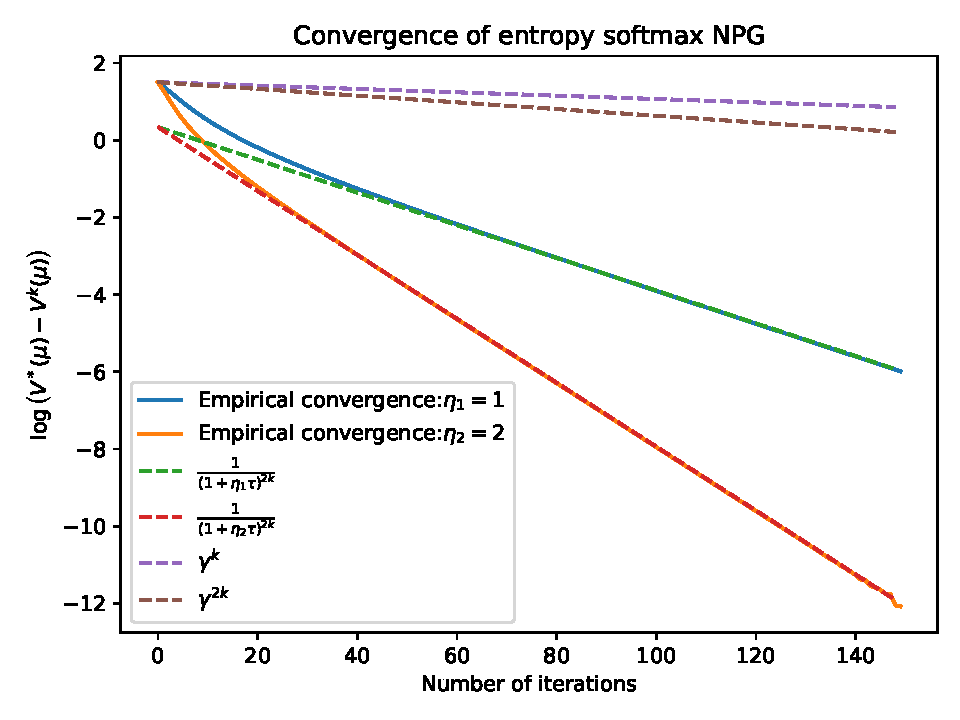
\includegraphics[width=0.45\textwidth]{EntropyNPG.pdf}
    \caption{Empirical justification of the local linear rate of entropy softmax NPG on random MDP with $|\mathcal{S}|=50$, $|\mathcal{A}|=20$, and $\gamma=0.99$: $\gamma$, $\gamma^{2k}$, and $\frac{1}{(1+\eta\tau)^{2k}}$ correspond to the limit convergence results presented in Theorems~\ref{theorem: ent_npg: linear convergence of log probability}, \ref{thm:entropyNPG-improvement} and \ref{thm:entropyNPG-local}, respectively. The regularization parameter is set to $\tau=0.05$ in the test.}
    \label{fig:entropynpg}
\end{figure}